\documentclass[12pt,a4paper,finnish]{tillbehor/tutthesis}
 
% LaTeX-tiedosto opinnäytepohjaksi
% Tekijä: Sami Paavilainen
% Muokkaaja: Heikki Huttunen (heikki.huttunen@tut.fi) 31.7.2012.
 
% Vaatii lisäksi luokkatiedoston tutthesis.cls
% sekä tiedoston tty-logo.pdf (pdflatex) tai tty-logo-eps (latex)

\usepackage[utf8]{inputenc}

\usepackage[small]{caption}% kuvatekstien kirjasinkoko ja asettelu
%omia käskyjä voi lisätä tähän väliin, esim. \newcommand{\angs}{\textsl{\AA}}
\pagenumbering{Roman}
% alkuvalmistelut loppuu
 
\begin{document}

 
\thispagestyle{empty}
 
\vspace*{-.5cm}\noindent
 
% If thesis is in English, use the file "tut-logo"
% instead of "tty-logo" in the following:
 

\includegraphics[width=8cm]{tillbehor/tut-logo}
 
\vspace{6.8cm}
 
\noindent{\bf\large \textsf{Mikko Pohja}}\\
{\bf\large \textsf{Maximizing quality in a small budget software project}}\\
\textsf{Master of Science Thesis}
 
\vspace{8.7cm} % jos kaksi otsikkoriviä vaihda -> 6.7cm
 
\begin{flushright}
  
\begin{minipage}[c]{6.8cm}
\begin{spacing}{1.0}
\textsf{Examiners: Tarkastaja 1}\\
\textsf{Examiners and topic approved in}\\ 
\textsf{the Information Technology}\\
\textsf{Department Council meeting on}\\
\textsf{xx.xx.xxxx}\\
\end{spacing}
\end{minipage}
\end{flushright}
 
\newpage
 
\setcounter{page}{1} % tämä tarvitaan, jottei ensimmäinen sivu kansilehden jälkeen olisi numero 2.
 
\chapter*{TIIVISTELMÄ}
\begin{spacing}{1.0}
\textsf{TAMPEREEN TEKNILLINEN YLIOPISTO}\\
\textsf{Tietotekniikan koulutusohjelma}\\
{\bf \textsf{Mikko Pohja: Maximizing quality in a small budget software project}}\\
\textsf{Diplomityö, xx sivua, x liitesivua}\\
\textsf{Xxxxxkuu 201x}\\
\textsf{Pääaine: }\\
\textsf{Tarkastajat: }\\
\textsf{Avainsanat: }\\
\end{spacing}
 
\noindent
Ensimmäinen kappale
 
\noindent
Toinen kappale
\newpage
\chapter*{ABSTRACT}
\begin{spacing}{1.0}
\textsf{TAMPERE UNIVERSITY OF TECHNOLOGY}\\
\textsf{Master's Degree Programme in Information Technology}\\
{\bf \textsf{AUTHOR : Title}}\\
\textsf{Master of Science Thesis, xx pages, x Appendix pages}\\
\textsf{xxxxxx 201x}\\
\textsf{Major: }\\
\textsf{Examiner: }\\
\textsf{Keywords: }\\
\end{spacing}
 
\noindent 
First paragraph
 
\noindent
Second paragraph
 
\newpage
 
\chapter*{PREFACE}
\noindent Tämä (\textit{d-tyo.tex}) on \LaTeX-pohja Tampereen teknillisen
yliopiston opinnäytetöitä varten. Samaan pakettiin kuuluu myös
tiedosto \mbox{\textit{tutthesis.cls}}, joka sisältää taittoteknisiä
lisäyksiä \LaTeX:n alkuperäiseen \textit{report.cls}-luokkatiedostoon.
 
Lisäksi otsikkosivua varten tarvitaan tiedosto \textit{tut-logo.xxx}, jonka
tulee sisältää TTY:n logo. Tiedoston tulee
olla joko \textit{.eps}- tai \textit{.pdf}-muodossa riippuen \LaTeX-versiosta.
 
\newpage
\tableofcontents
%\newpage
%\listoffigures
%\listoftables
\newpage
\chapter*{TERMS AND DEFINITIONS}
 
% Näitä ei välttämättä tarvi olla
\begin{termiluettelo}
 
\item [Life cycle] TODO
\item [Function point] TODO
 
\end{termiluettelo} 
 
 
\newpage
\renewcommand{\chaptermark}[1]{\markboth{\thechapter. \ #1}{}}
\renewcommand{\sectionmark}[1]{\markright{}{}}
\lhead{\fancyplain{}{\leftmark}}
 


% Tästä alkaa varsinainen teksti
\pagenumbering{arabic}
 

\chapter{Introduction}

%Konteksti
% Koodauskielien, frameworkkien, ympäristöjen (as a service) kehittyminen ja osaamisen lisääntyminen on tehnyt mahdolliseksi softan tekemisen ilman massiivista budjettia, suurta tiimiä tai pitkää prosessia.
% Lean ja Agile on helpottanut ja nopeuttanut kehitystyötä ja tehnyt mahdolliseksi nopean validoinnin ja julkaisemisen.
% 

Progress in recent history has made developing new products and services in the field of software development increasingly easy. New and improved programming languages and frameworks are introduced constantly. These frameworks provide easy to start platforms for new software development removing the need for excessive planning and understanding of many low-level implementation details. In addition, the need for expensive hardware setup has come obsolete as several instances have appeared offering reasonably priced execution environments as a service. 

These changes in the industry along with the progress in development processes have brought the possibility to create software business closer to every would-be entrepreneur. Developing software with Agile or Lean methodology with modern technologies have lowered the initial time and resources required. Experienced software developers can implement a prototype as fast as in weeks starting from scratch and ending in having a working product publicly available. Attempts to create the next big software product are on a rise as the stories of success spread around the globe.

% TODO: lisää kontekstia?

%Ratkaistava ongelma
% Helppo ja nopea tekeminen johtaa helposti huonoon laatuun sekä budjetin ja aikataulun kasvuun
% 

Since the number of attempts for success are increasing, so is the number of companies succeeding. When a product built with minimum effort starts to prosper, the demand for high quality emerges. As products done by traditional software development are built with large amounts of effort used to improving the quality of the product, modern startup entrepreneurs may become confused when considering the quality of their product. The methods and activities used in traditional software development may seem separate from the rapid development of modern products. In addition, modern software development methodologies focus on different aspects of software quality than in traditional software development.

%"Tässä diplomityössä..."
% Käsitellään perinteisiä laadunvarmistusmenetelmiä sekä niiden tehokkuutta
% Kerrotaan startupista yleisesti sekä sen määritelmästä laadulle
% Kerrotaan perinteisten laadunvarmistusmenetelmien soveltumisesta nykyisiin startupin juttuihin
% Käsitellään esimerkkinä CASE-projekti, joka on pienehkön budjetin projekti startupille

This thesis presents software quality in a startup environment and suggests the activities for improving it. Traditional quality improvement methods are presented and linked to the methods recommended in startup environments. Also a real-life software project for a Finnish startup is presented for illustration purposes. The project, executed in a Finnish software company Futurice, is evaluated by using the data gathered after the project from interviews of the project stakeholders.

%Rakenne luku kerrallaan + sisällön esittely "lause per luku"

The rest of this thesis is organised as follows. Chapter 2 introduces the background by defining software quality and startup environment. Chapter 3 describes the methods and activities improving software quality and divides them in phases of traditional software development. Chapter 4 redefines quality in context of a software startup and describes the methods of quality improvement applicable in startup software development. Chapter 5 presents the execution and phases of the case project and evaluates the quality achieved based on the interviews of the stakeholders.

 
 %%%%%%%%%%%%%%%%%%%%%%%%%%%%%%%%%%%%%%%%%%%%%%%%%%%%%%%%%%%%%%%%%%%%%%%%%%%%%%%%%%%%%%%%%%%%%%%
 SOFTWARE QUALITY
 %%%%%%%%%%%%%%%%%%%%%%%%%%%%%%%%%%%%%%%%%%%%%%%%%%%%%%%%%%%%%%%%%%%%%%%%%%%%%%%%%%%%%%%%%%%%%%%
 
 
 \chapter{Software Quality}
 
This chapter describes software quality and methods for improving quality in software projects. The first section describes software quality in general and the motivation behind improving quality. In the second section the most popular active and passive methods for improving quality are introduced.

 \section{Software quality in General}
 
\subsection{Software quality defined}

Quality is an attribute of the item in question. It is often described as a combination of qualitative and quantitative attributes. Quality is an ambiguous attribute, because it is subjective and thus differs when viewed from different perspectives. American Society for Quality has two definitions for technical quality: 1. the products ability to satisfy its needs; 2. the products lack of deficiencies~\cite{ASQglossary}

% Subjektiivista
In software business, quality has also multiple viewpoints. Quality has different meanings for vendors, customers, end-users etc. 

% ECO: Chapter 1
 
% Haikala s.48: toiminnan laatu vs tuotteen laatu

% Haikala s.49 verification/validation 'tehdäänkö tuotetta oikein' ja 'tehdäänkö oikeaa tuotetta'

% mittaus

% http://ryreitsma.blogspot.fi/2011/07/software-has-new-quality-model-iso.html
% Virallinen, ISO 25010: Functional suitability, Reliability, Operability, Performance efficiency, Security, Compatibility, Maintainability, Transferability

% tavoitteena luoda arvoa asiakkaalle

\subsection{Motivation}

% \ Chapter 1, software has become..
Software is one of the most used type of product in human history. At the same time it has one of the highest failure rates of any type of product mainly due to poor quality. With those facts, it is clear that the total influence of low quality software is considerable in both money and time. Still it is a known fact that a common practise to cut costs is reducing the effort used in software quality. Convincing the payer to allow using effort to achieve good quality can be difficult but crucial. The topic is widely researched and the results speak in behalf of quality.

Phil Crosby has made popular a concept that establishing a quality program will return in savings more than the program costs and thus "quality is free" [VIITE Quality is free]. Even though Crosbys concept is used mainly in manufacturing sector, it has some truth that can apply to software business.  In addition, the "cost of quality" is a slightly inappropriate term, >considering that quality in itself doesn't create costs but the lack of it. 

%\ Cancellation 31\% for 10000 function point projects. Costs 35M\$ vs high quality 20m\$
Studies have shown that software quality has huge impact on project costs and success. Measurements on 10000 function point projects show that about 31\% of projects that size come to an end by cancellation. The average cost of these cancelled projects is about \$35,000,000. Succesfull projects the same size with good quality have about 40\% lower costs. These figures endorse the effort put to the software quality and make it clear that at least in large scale projects, quality control shouldn't be ignored.

% ECO: page 19 Reduces the odds of large-system cancellations, Shortens development schedules, Lowers development costs, Lowers maintenance costs, Reduces warranty costs, Increases customer satisfaction
Capers Jones has listed several points that make high quality a major enocomic benefit. In the development of large systems, high quality from the beginning can reduce the propability of cancellations. Software projects can also benefit by achieving shorter development schedules. Shorter schedules with high quality also lowers the costs of a project. Lower development costs, maintenance costs and warranty costs can add up to considerable amounts of cost savings. In addition to the quantitative benefits, high quality raises the satisfaction of customers, end-users and developers. 

% ECO: it is gratifying to observe that high quality levels are invariably associated with shorter-than-average development schedules and lower-than-average development costs
Jones expresses concerns towards the poor measurement of software quality causing executives and even quality personnel to treat software quality as an expense. Those participants may also treat quality as an issue that is raising the development costs and increasing development schedules. As an equivalent, Jones summarizes the benefits of high quality: "However, from an analysis of about 13,000 software projects between 1973 and today, it is gratifying to observe that high quality levels are invariably associated with shorter-than-average development schedules and lower-than-average development costs"~\cite{jones2011economics}

 
 
 
 


%%%%%%%%%%%%%%%%%%%%%%%%%%%%%%%%%%%%%%%%%%%%%%%%%%%%%%%%%%%%%%%%%%%%%%%%%%%%%%%%%%%%%%%%%%%%%%%
	QUALITY ASSURANCE IN STARTUP SOFTWARE PROJECT
%%%%%%%%%%%%%%%%%%%%%%%%%%%%%%%%%%%%%%%%%%%%%%%%%%%%%%%%%%%%%%%%%%%%%%%%%%%%%%%%%%%%%%%%%%%%%%%
 

 \chapter{Improving Quality in Software Startup Project}

This chapter describes the differences between quality improvement in traditional software development and modern software startup. First, the meaning of software quality is redefined in a startup environment. Second, the basis of quality and the activities improving quality in a startup environment are described. Third, the activities from traditional software development are linked to the activities used in modern software development. Finally, the practices used in the company responsible for case project described in the next chapter are introduced.



% Laatu painottuu startupissa siihen, mitä asiakkaat ja loppukäyttäjät pitävät tärkeänä
% Laadun merkitys elinkaaren eri vaiheissa muuttuu
%	-Aluksi tärkeintä validoida featuret ja idea
%	-Laadussa tärkeää aluksi hyvä muokattavuus, refaktoroinnit, asiakkaalle kriittisten osien testaus
%	-Elinkaaren alussa ei väliä matalan prioriteetin bugeilla tai featureiden vajaalla toiminnalla
%	-Kun idea alkaa olla validoitu, muuttuu laadun merkitys tuotteistuksen yhteydessä
%	-Laatuun on käytössä myöhemmin enemmän resursseja, koska asiakkaita alkaa olla
%	-Osuiskohan tähän Lean Startupin skaalausvaihe

 \section{Quality in a Startup project}

In the beginning of the chapter about role of quality, Eric Ries states that "The best professionals and craftpersons alike aspire to build quality products; it is a point of pride". This is a good summary about the attitude towards software quality in many movements about modern software development. Measuring and defining quality in modern software projects with constant changes and uncertainty can be difficult, but the development personnel should have the pursuit for high quality.

Ries tells that modern production processes seek to boost efficiency by relying to high quality. The belief that the customer is the most important part of the production process means that all effort should be focused to producing results that the customer finds valuable. This view can be beneficial in an environment where the company knows the opinions of customers. However, in a startup development, assuming the opinions of customers is a risky thing to do. Often in the startup, it is not even sure who the customer is. Thus, Ries introduces a quality principle for startups: "If we do not know who the customer is, we do not know what quality is".

In a startup developing an MVP, the quality of the product can be a fluid concept. Even if the quality of MVP is low for customers, it can bring great value in building a high-quality product. If the customers find the product low on quality, this can be used as an opportunity to learn what customers care about. This is infinitely better than mere speculation, because it provides empirical information on which to build future products.

When working with a 3D chat software called IMVU, Ries and his colleagues decided to leave a critical sophisticated feature done with only minimum effort. They were embarrassed to release the moving of the avatars without any animations or other modern visualizations. The avatars just reappeared to another location. The response of the customers was surprising as the customers were thrilled from the new feature, which allowed an immediate change of location without waiting. From the customers point of view, the released feature was more appropriate than the option which would take more time and money to implement. In the end, the quality of the released feature was probably higher than the one planned. The lesson behind the story is that customers do not care how much time something takes to build.

Lean Startup method is aiming for the goal of winning over customers and not opposed to building high-quality products. Thus, it is necessary to set aside some professional standards to enable the validated learning as soon as possible. This is not supposed to allow operating in an undisciplined manner. This is important as there are some quality problems that can slow down the Build-Measure-Learn feedback loop. In addition, defects complicate the evolution of the product and interfere with the ability to learn. Helping the development of the MVP means removing any feature, process or effort that does not lead directly to the learning sought.~\cite{ries2011lean}

\section{TODO: Foundations of high quality}

 \subsection{Clean code} 

 Every programmer with experience for more than two or three years have probably been slowed down by messy code. Over a couple of years of development, teams that were moving fast at the beginning of the project can be slowed down to a really slow pace. Development begins to include more and more non-trivial changes, which are about resolving the existing knots and tangles and adding new. Eventually, the mess can become so big that it can not be cleaned up at all. The total cost of owning a mess is being pondered by Robert C. Martin in his book Clean Code: A Handbook of Agile Software Craftmanship.

 Martin reminds that "code is really the language in which we ultimately express the requirements" and thus code is in the very foundations of every software project. A common mistake done in software projects is to increase the measure of developers in the team. This is usually done when the code has already reached a too messy state and the pace of development has slowed down. Adding new staff to the development does not improve the situation, but underlines the meaning of messy code. This new staff is not familiar with the existing system, so they easily complicate the system even further, driving the productivity even worse.

 A bitter fact for the developers is that usually the cause of messy code is the fault of the developers. While the management and sales staff are defending schedules and requirements, the developers should be defending the code. Many developers previously slowed down by messy code still feel the pressure of deadlines and the temptation to make messes to achieve them. Martin says that true professionals know that the only way to go fast is to keep the code as clean as possible at all times. A programmer able to write clean code is an artist, who can use all the little techniques in a disciplined manner through the sense of cleanliness.~\cite{martin2008clean}
 
 \subsection{Integrity} 

 One of the principles of Lean Software Development (LSD) is "Build Integrity In", which has its premises in high-performing automotive companies in 1980s. A study "Product Development Performance" by Kim Clark found out that the product integrity was a key difference between average and high-performing companies in developing superior products. Clark found out that integrity has two dimensions: external integrity and internal integrity.~\cite{clark1991product}

 LSD renames these two types of integrities as perceived integrity and conceptual integrity. Perceived integrity is a balance of function, usability, reliability and economy observed by the customer. It is affected by the whole experience of the system beginning from advertising and delivery to intuitiveness and the ability to solve the problem. An analogy to the measure of perceived integrity comes from the question: which ones of the bookmarks of your browser would you add back immediately, if you wiped out them all? These are the products with perceived integrity. 

 Conceptual integrity is smoothness and uniformity of the whole system's central concepts. The architecture of the system has an effective balance between flexibility, maintainability, efficiency and responsiveness. Conceptual integrity is a prerequisite to perceived integrity. To be able to achieve perceived integrity, the system must have a consistent design. As the system evolves and matures, conceptual integrity emerges. Although conceptual integrity is needed for perceived integrity, the existence of the former does not ensure the existence of the latter. This is because conceptual integrity is not sufficient for a successful customer experience, if the system does not meet the users' need.~\cite{poppendieck2003LSD}

\section{TODO: Aiming towards high quality}

\subsection{Build Integrity In} 

In the study by Kim Clark, a primary claim is that integrity is achieved through superior information flow. Perceived integrity is a projection of the integrity of the information flow between users and developers. In turn, conceptual integrity is a projection of the integrity of the upstream and downstream of technical information flow. When reaching a system with high perceived and conceptual integrity, an excellent information flow is necessary both between customer and development team and between the upstream and downstream processes of the development team. Information flows must take into account both the current and potential uses of the system.

\textbf{Perceived integrity.} In traditional software development, perceived integrity is transmitted to programmers through a multistage process. In this process, requirements are collected and processed through analysis and design. Then the design is transfered to the programmers implementing the code. These multiple hand-offs will cause the loss of considerable amount of information, key details and future perspectives. Fortunately, an alternative for this multistage process is to establish a superior customer-developer information flow by other means. With smaller systems, the development should be done by a single team having direct access to the people capable of judging the systems integrity. This team should use short iterations in where the system is demonstrated to a wide range of people giving feedback about the integrity. This way the feedback can be used for a rapid steering of course. Another technique is to use customer tests purposely created for getting feedback.

% Communicating two-ways face to face in small batches and solving the problems at the same time
\textbf{Conceptual integrity.}
Conceptual integrity in automotive manufacturing is pursued by using existing parts and integrated problem solving. In integrated problem solving, understanding and solving the problem happen simultaneously, instead of sequentially. The initial information is released early and not only after complete information is available. Information flow happens in two directions instead of one and it contains multiple small batches of information instead of a single large batch. The preferred communication style is face to face instead of documents. This kind of problem-solving is ideal for achieving conceptual product integrity, particularly in development of complex systems such as automobiles or software systems.

In software development, using integrated problem solving means that the development must be started before the design is finalized. In addition, the developers should be able to access customers or customer representatives for getting the answers as soon as possible for any questions raised. Customer tests should be developed and ran along the iterations and not just at the end.

Finally, using experienced developers in their own areas of expertise can help in achieving conceptual integrity. Not all of the developers have to be with plenty of experience, but for the complex areas, experience brings understanding of the technical details and patterns widely used to manage with the complexities. One of these experienced developers should be a master developer facilitating the effort over multiple teams. For example, integrating the decisions and trade-offs among multiple developers and customers would be the responsibility of the master developer.

\textbf{Refactoring.} When the integrity of a product is building, the iterative development brings continuous improvement as the product is evolving. In software development, the system must be continuously improved by the developers. Otherwise the internal structures of the software will become calcified and fragile. In time, the system will even stop working. Refactoring is done to prevent this disintegration of the software structures over the development.

The need for refactoring comes when new features are added to the system one at a time and the architecture and requirements of the system change gradually. Often it would be better to think of new related features as a set and build an architectural capability to support them. If the features are added in multiple different locations of the code, the system will lose conceptual integrity. Refactoring regularly keeps the system healthy.

TODO: p. 142-144

\textbf{Testing.} In a traditional software development where implementation is done single module at a time, there are numerous types of testing used. There are for example unit testing, system testing, integration testing and acceptance testing used. The purpose of testing is to check that the intention behind the design is achieved and the system does what the customers want it to. In LSD, the development is done by implementing entire features instead of single modules, so the distinction between the different kinds of testing is more artificial. Instead, testing is divided into two parts: developer tests and customer tests. Developer tests are testing that the implemented features work as intended and that all the pieces work together. Customer tests are developed to verify that the system does what customers expect.

Tests act in several different roles in the development process. First, they present the exact functioning that the features are supposed to have. Second, they also supply information on whether the features actually work as supposed. Third, tests act as a scaffolding which provides support for tools such as refactoring. This allows the developers to make changes during the development. Fourth, after the development is done, the tests provide a representation of how the system was built. Finally, developing sufficient tests for all systems in production, making changes to these systems can be verified by running the tests for all related applications.

Tests can also work as a tool for communication. Customer tests can be written within the conversation with the customer about details of desired functionality. This way the tests can give the most accurate description of how the features should work for a customer. Likewise, developers can document the planned design by writing tests testing exactly what the design should do. There are other tools allowing the communication before the code is written, but there is no substitute for testing whether the system does what it is supposed to do. With this in mind, using tests for both tasks can be beneficial.

Receiving immediate feedback about the correct operation of code is important to a developer. The developer usually somehow tests the code as soon as its written, so the test could be captured as a written test allowing the reuse. Another opportunity to catch necessary experiments as tests is the review to customer within an iteration. Demonstrating the current system to a customer can be done with a set of demos or scripts, which can be captured as customer tests. These captured tests should be run as often as possible, so the team should ensure that the tests will not take too much time and are automated as much as possible.

Using automated testing with extensive test suites for both developer testing and customer testing can be an efficient way to implement scaffolding to support the development. The scaffolding is a structure supporting the developers when they are making major changes to the system. While developing software in iterations, refactoring and other tools will include changes, which tend to have unintended effects. Having these effects in the system without the scaffolding provided by automatic tests can be an unsustainable situation. Often it may seem that writing tests slows down the development, but it pays back both during development and over the systems life cycle.

\subsection{Empower the Team}

Lean thinking emphasized the importance of intelligent, disciplined and motivated frontline workers. In LSD, it is believed that the critical factor in motivation is empowerment. This means moving the decisions to the lowest possible level in the organization while assuring that those people have the ability and resources to decide wisely.

%\textbf{Self-Determination.}
% Nummi

\textbf{Motivation.} 3M is a company which is regularly meeting its goal that 30\% of each divisions sales is generated by products introduced in the last 4 years. This stream of new products has been keeping the company continually renewed for over 75 years. In the core of the company is a formula that allows the entrepreneurial spirit prosper. This vision includes that the heart of the company consists of small, self-organizing groups who are passionate about a possibility and are allowed to realize the possibility. This kind of invention forms a company which evolves from the creativity of the individual employees rather than from the planning of managers.

In the book Lean Software Development, roots of motivation are described as follows: "Insintric motivation comes from the work we do, from pride in workmanship and a sens of helping a customer." Intrinsic motivation is specifically strong in a team which has a commitment for reaching towards a purpose the team cares about. 

The sense of purpose can be achieved with several ways. In the beginning, there should be a clear and compelling purpose. This compelling purpose brings commitment and passion for bringing out the product. The purpose should be achievable. It should be made sure that the team has the capability and resources required for accomplishing the goal within itself. The team should be able to access the customers. Communicating with real customers can help understanding the purpose and also give insight into their individual work.

The team should make its own commitments. The amount of work fitting into the iteration should be a call made by the team. Commitment in a team is a commitment to each other. Managements role is to remove interference. A leader does not need to tell a motivated team what to do, but listen for how the team could advise the leader. This helps the leader to remove obstacles and thus maintaining the momentum of the team. The team should not have skeptics around, because people who know plenty of reasons why things cannot be done, can kill the purpose really fast.

There are four building blocks of motivation. First, a feeling of belonging can be achieved in a team where members are equal and respect each other. Having winners and losers created in the team can seriously harm the feeling of belonging. Second, feeling of safety is about the atmosphere of making mistakes. Tolerating no mistakes will kill all initiative as in creative processes tolerance of mistakes cannot be zero. Third, a sense of competence comes from success in challenges, positive feedback, knowledge and skill. In addition, a good leader must justify that the team is on a right track and having the resources needed to be successful. Finally, sense of progress will be maintained when the team has the feeling of accomplishment. Developing software in iterations is supporting this feeling as in every iteration the team gets to put its work in front of the customer for feedback.

There are some downsides in passionate attitude towards a purpose. First, long working days and nights can be productive for a some time, but they are not a part of sustainable working culture. Second, different levels of passion are to be found inside teams. This means that there is a risk that the members of a team are expected to work long days. It is not fair for those not choosing them voluntarily and this can affect the spirit inside the team.

\textbf{Leadership.} Innovative teams at 3M are led by a passionate leader called "product champion". This leader is usually the person behind the initial product concept. Getting support from the management and forming the team are also in most cases done by this leader. The leader is supposed to represent the customer by interpreting the product vision to the team. In Toyota, there is a similar position called "chief engineer". He has complete responsibility for the vehicle and the power to make all the decisions. It is common in these positions that the product is named after the bearer of this position. Another similarity between these companies is that these leaders do not have direct authority over the people working in the team. They are the leaders of their teams, not managers. In LSD, these respected leaders are called "master developers".

The position of a master developer is not usually designated, but it is emerged. It is not necessary that there is a known master developer in the beginning of a project. A person with deep experience and understanding on both technical and customer issues usually rises to this position. Master developer is part of the team working towards the purpose and empowering the team. Architects and other advisory roles are not likely in a role of master developer, because they are not a part of the team.

\textbf{Expertise.}

In software development, there are two major areas of expertise: technical knowledge and domain knowledge. Technical knowledge creates experts in areas such as database administration, user interface design and embedded code. Domain knowledge includes understanding of the domain of the business, for example health-care or security.

Expertise in different areas evolves best in communities of expertise, where people responsible for same kind of activities meet. A traditional method of developing these communities inside a company is to divide the company into functions by core competence. These functions can include program leaders guiding the teams in product development. This structure is called a matrix organization.

In a successful matrix organization the two managers each person has, view their jobs correctly. Functional managers should act as mentors and teachers. They should supply the inexperienced members of the team with support and coaching through progressive series of assignments. Value adding managers should view their jobs as enablers and motivators who remove impediments and supply resources to the team.

Companies not using matrix organization should also preserve communities of expertise. These communities can be gathered by identifying the areas of competence in both technical and domain knowledge. The members in formed communities should be available for communication and information sharing using repetitive meetings or other media reaching everyone in the community. If the amount of experts in a critical area is not sufficient for forming internal community, external communities are usually available for support in the expertise.

% \subsection{TDD}

% \subsection{Iterative development}
% p.27

\subsection{Activities}

\textbf{Pretest.} Activities used in pretest defect removal were studied and presented by Capers Jones in The Economics of Software Quality. The study was aimed at small software projects and the results divided the defects found by the origin of defect and the activity it was found with. Defect origins distinguished were requirements, design, code and documentation. Used activities were desk check, scrum, client reviews, peer reviews and static analysis. The results show that over half of the defects were found from the code. The most effective activity for finding the defects prior to testing was static analysis. Considering the almost automatic nature of static analysis, it can be seen as a predictable result. The results presented in Figure~\ref{fig:pretest-efficiency} can aid in choosing the pretest defect removal activities.\cite{jones2011economics}

\begin{figure}[t]
\begin{center}
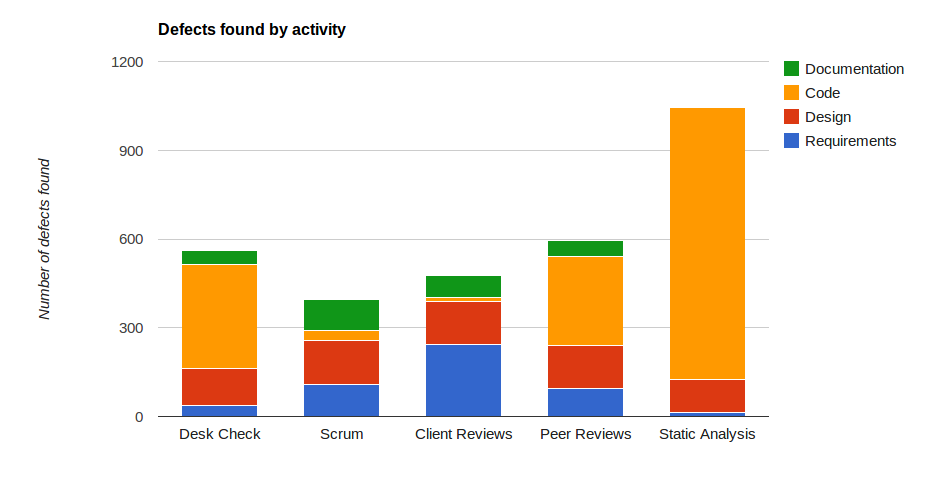
\includegraphics[width=1.0\textwidth]{image/pretest-efficiency.png}
\end{center}
\caption{Efficiency of pretest defect prevention}
\label{fig:pretest-efficiency}
\end{figure}

\textbf{Defect prevention.}


\textbf{Testing.}


% PREVENTIVE
% -Small business applications p.126
% 	-1000fp
% 	-embedded users
% 	-agile development method
% 	-TDD
% 	-automated risk analysis
% 	-static analysis on all code segments
% -This combination should lower defect potentials by 45\% and ensure defect removal 95\%

% ECO: We use these quality metrics to compare a number of quality improvement techniques at each stage of the software development life cycle and quantify their efficacy using data from real-world applications.
 
% Direct costs \& efforts p. 200 table
% ECO: Analysis of pretest defect removal activities p. 208
 
% DEFECT TRACKING IS A WASTE

%http://books.google.fi/books?id=RTt9AgAAQBAJ&lpg=PA27&ots=PXXKjr2e_E&dq=%22According%20to%20Shigeo%20Shingo%2C%20there%20are%20two%20kinds%20of%20inspection%22&pg=PA29#v=onepage&q&f=false
% In Lean Software Development, the goal is to build quality into the code from the start, not test it in later. Dont focus on putting defects into a tracking system, you avoid creating defects in the first place. It takes a higly disciplined organization to do that. p26
% There are two kinds of inspections, inspection after defects occur and inspection to prevent defects. If you really want quality, you don't inspect after the fact, you control conditions so as not to allow defects in the first place. If this is not possible, the you inspect the product after each small stemp, so that defects are caught immediately after they occur. When a defect is found, you stop the line, find its cause and fix it immediately. p.27
% Defect tracking systems are queues of partially done work, queues of rework. In Lean, queues are collection points for waste.

% {poppendieck2006implementing} 



\section{The Don'ts - Things To Avoid}

% Liittyy vahvasti Leanin Wasteen
% Älä raportoi bugeja, joista tiedät, ettei niitä korjata
% Ei turhia raportteja
% ECO: Cost per defect => paras tulos bugisimmassa projektissa
% ECO:  p. 127 harmful combinations PREVENTIVE

% Right the first time LSD p.19(?)

Capers Jones has interpreted from the research of multiple years of software quality that there can be harmful combinations of methods used. Even when combinind harmful methods with helpful ones, the harmful method seem to end up winning. That is, defect potentials are raising instead of coming down. Some methods combined with others can raise the defect potentials and make applications risky with a change of failure.



 \section{Software Quality in Futurice}
\label{sec:quality_futurice}

% http://www.futurice.com/wp-content/uploads/2014/02/Fact-Sheet-English2.pdf
Futurice is a lean service creation company founded in Finland. There are currently around 200 employees in four offices located in three countries. The employees of the company are passionate multi-talents in areas from technology, business consultancy and service design.~\cite{futuricefact}

Futurice does not have strict processes or common practices in quality assurance. The main idea present in all activities in the company is that smart people make smart decisions. With software quality, this means that the developers and other members of the project teams are able to decide their own approach to software quality. This freedom of choice leads to experimentation of multiple activities and practices, from which the good and bad experiences can be shared with others. Some practices of course become more common than others, but the use of those is not forced in any way. A common way of executing projects is to use methodologies from Lean and Agile software development.

In the core of Futurice, is communication and transparency. All the decisions and experiences are available for everyone and this brings the possibility to make decisions to every employee in the company. There are also informal communities built for areas of interests, such as mobile development and web development. These communities have recurring events where experiences are shared.

For the longer-term projects there is a separate team named Life Cycle Management team. Members from this team are present in a project from the beginning and they live through the product's life cycle participating in the development and maintenance of the product. This ensures that there is a solid amount of experience present in the team from the beginning of the project to the post-release phases.

 
%%%%%%%%%%%%%%%%%%%%%%%%%%%%%%%%%%%%%%%%%%%%%%%%%%%%%%%%%%%%%%%%%%%%%%%%%%%%%%%%%%%%%%%%%%%%%%%
	CASE
%%%%%%%%%%%%%%%%%%%%%%%%%%%%%%%%%%%%%%%%%%%%%%%%%%%%%%%%%%%%%%%%%%%%%%%%%%%%%%%%%%%%%%%%%%%%%%%


 \chapter{Case: Päikky}

This chapter presents phases from a project done before the writing of this thesis. The execution of the project was done with no intention of it being a part of a thesis work. All the data shown here are gathered afterwards and thus do not meet the requirements of a proper scientific study. The project is presented here as an example project of a small budget startup.


 \section{Project objectives}

The project was built on an idea from MukavaIT. The big picture and the goals of the project were specified in advance and introduced to the developing team. Lower level specifications and implementation details were designed in cooperation between MukavaIT and the development team.

The objective of the project was to create a new kind of recording system for kindergartens. The system would allow the tracking of the arrival, departure and absences of the children in the groups. The main goal was to make a user-friendly system which connects parents, employees of the kindergartens and the administrative personnel in the municipality. The connection between the stakeholders would enable the planning of the need for day care and the real-time tracking of the nurses and children. The eventual goal of the system would be the dynamic hour-based billing models. In addition to this, the system would produce several types of reports for the administrative personnel for optimizing the daycare system.

The most important functionality of the system would be that the nurses are able to record the presences of the children with mobile devices. The recordings will be collected to a database serving different services for nurses, parents and administrative personnel in the kindergartens. The services would include a mobile client for nurses, a desktop client for parents and another desktop client for administrative personnel. A common goal in which these clients are aimed at, is to bring the daycare system towards a genuinely transparent process, which encourages the parents to participate more in the early childhood education.

During the development, a better understanding of the market was achieved. It was learned that reaching towards the hour-based billing models and the report generation was not as necessary as it first seemed. The stakeholders became interested already as the first version of the system was released into pilot use. The features that allowed the parents to communicate with the nurses were something the parents were excited of. In addition, the recording and checking the presences, communicating with the parents and storing the information about the children all in the same system were inspirational for the nurses.

This understanding of the market was not present when deciding the priorities of the upcoming features, so some of the effort put to reporting and other features could have been allocated to more appealing features.

 \section{Team and Phases}

The project was divided into multiple phases. In the scope of this thesis, five phases are observed. Each of the phases had a couple of predefined objectives and a schedule.

% http://www.qsm.com/resources/function-point-languages-table
% Function points

% ensimmäinen MVP
% pieni ja yksinkertainen
% kokeilut, testausta siirrettiin tulevaisuuteen
% featuret edellä, testaus jälkikäteen
% asioiden validointi, epäselvät speksit -> tuntui turhalta testata ilman tietoa onko toiminnallisuus järkevää



% -Kerrotaan prosessista ja tiimistä 



% * Vaihe 1
% 	* Aikataulu: 20.11.2013-15.2.2013
% 	* Budjetti: 66 690€ (60 000€)				26%
%	* Function points 				130 (+130)
% 	* Pääkontentti: 
% 		* Lasten ja hoitajien läsnäolon mobiilikirjaus
% 		* Admin UI päiväkotien, ryhmien, lapsien ja hoitajien tietojen syöttämiseen
% 	* Tiimi
% 		* Osmo
% 		* Mike
% 		* Antti
% 		* Jouni
% 		* Elice
% * Vaihe 2-3
% 	* Aikataulu: 19.2.2013-4.6.2013
% 	* Budjetti: 56%   144 840€ (136 000€)
%	* Function points 				415 (+285)
% 	* Pääkontentti: 
% 		* Kommunikointi päiväkodin ja kodin välillä
% 		* Hoitosuunnitelmat
% 		* Päiväkodin käyttöliittymä tietojen selaamiseen ja muokkaukseen sekä raportointiin 
% 	* Tiimi
% 		* Osmo
% 		* Mike
% 		* Kalle
% 		* Mikko (huhtikuu ->)
% 		* Elice
% * Vaihe 4
% 	* Aikataulu: 5.6.2013 - 15.7.2013
% 	* Budjetti: 6%   15 000€
%	* Function points 				475 (+50)
% 	* Pääkontentti: 
% 		* Perhepäivähoidon toiminnot ja rajapinnat 
% 	* Tiimi
% 		* Osmo
% 		* Mike (osa-aikainen)
% 		* Miro
% 		* Kimmo
% 		* (Elice)
% * Vaihe 5
% 	* Aikataulu: 15.7.2013 - 16.7.2013
% 	* Budjetti: 12%   30 000€
%	* Function points 				500 (+25)
% 	* Pääkontentti: 
% 		* Läsnäolotietomallin uudistus, läsnäolotietojen esitys ja muokkaus, kulukorvaukset kunta UI:hin 
% 	* Tiimi
% 		* Osmo (osa-aikainen)
% 		* Mike
% 		* Miro
% 		* Kimmo
% 		* (Elice)





 \section{Quality in the project}

Quality assurance in the Päikky project was not formally specified or planned beforehand. Methods and processes were selected primarily by individual developers and talked through with the whole team. Methods and tools were taken to use when necessary.

\subsection{Quality Methods and Processes}

\textbf{Agile development.} The project was executed using agile development. The development was done in a week long sprints, which included a weekly review and planning session. The customer representatives were present in the weekly meetings. This enabled that the implementation of the features in the finished sprint could be assessed against the understanding of the customer. 

\textbf{Static analysis.} The development of the application was mostly done by using some integrated development environment (IDE), although some of the developers involved in the development used only a source code editor without any intelligent features. These modern IDEs provide automatic tools for running continuous static analysis of source code. Using this kind of static analysis tool can prevent some defects from getting into the application. 

\textbf{Peer reviews.} With some parts of the application, ad hoc informal peer review sessions were used. These reviews were done in situations where the developer responsible for the implementation of a component had questions about the implementation details. In these brief discussions, parts of the code and thoughts about the implementation were reviewed by another developer. The end result of these session would usually be either an actual decision about the implementation or a joint decision that these details must be discussed with the whole development team or with the customer.

\textbf{Testing.} During the project, testing was one of the most problematic forms of quality assurance. In the beginning of the project, all the testing was done manually by using the system via the user interface. The effort for implementing the automatic tests were postponed in favor of the development of new features. Some critical features in the backend were tested with integration tests and a set of user interface tests were implemented during the first two phases of the project. However, in later phases the user interface tests were disabled because of the problems with the test runner. Alternative options for test runner were investigated, but no good enough solution was found with the effort put into the studies. Also the amount of integration tests did not increase at the same pace as the number of critical features. The attitude towards testing was not neglecting, but the amount of new features to implement did depress the allocation of effort on the testing.

% Preventing
%	agile, embedded users, static analysis
% pretest
%	peer reviews, scrum sessions, client reviews?
% testing
%	unit testing, system testing, 
% post-release
%	latent defects

% -Käytetyt QA-metodit
% -Static code analysis (IDEn vakiot)
% -Communication ("embedded users")
% -Testing(frontend, backend unit testing and integration tests)
% -Occasional reviews (rarely)
% -Continuous Integration


% Alkuun testattiin pelkästään UI:n kautta
% Testaus hiipui projektin myötä -> ei “riittävää” testausta
% Bäkkärin integraatiotestit -> testattiin kriittisimpiä osia, muttei kaikkia
% Satunnaisia testejä
% Automaattiset testit jumiin CI:ssä -> aikaa käytettiin korjaukseen, mutta ei onnistunut -> Testit % pois käytöstä
% Testit koetaan tärkeiksi
% laajuus kasvaa, joten ei tiedä miten asiat toimii 
% regressio uusien featureiden kanssa
% turvaverkko
% tekijät vaihtuu
% testit valmiita esimerkkejä oikeasta käytöstä/toiminnasta
% testien dokumentointi, ei tiedetty mitä testit testaa -> väärä luottamus
% TDD käytetty satunnaisesti bugien korjauksissa

 


 \section{Achieved Quality in The Project}

 The quality achieved in the project was evaluated by interpreting the views and opinions of the product stakeholders. A separate informal interview sessions were arranged with the development team, project manager and the customer representatives. In addition, notes from a retrospective session after the fifth phase were considered.

\subsection{Development Team}

The overall feeling of the development team was that there should have been more effort put into the quality assurance during the project. The actual development suffered from the lack of effort put into the quality aspects. The shortage of testing and other methods of quality assurance seemed to affect negatively more and more as the project advanced. 

\textbf{Testing.} Testing was one of the most important themes brought up in the interviews with the development team. In the beginning of the project, testing was taken into consideration and some effort was put into bringing testing tools in use. Testing tools for testing both the backend and frontend were studied and selected. Some tests for testing the most critical features in the backend were written through the whole project. For the frontend, only a few tests were written and the execution of those tests were unstable from the day one. The final setback for the frontend tests was got when the chosen test runner began to freeze during the execution of the tests.

Biggest problems with testing was that there were no common practices or clear allocation of effort to the writing of the test cases. According to the understanding of the development team, there were defects present that could have been prevented with proper tests. The general feeling was that putting more effort to testing would have helped save time and money.

Proposals for improving testing suggest that in the first place, the infrastructure for the testing should be repaired. The test runners should execute the tests reliably and the tests should be run in the CI environment. In addition to fixing the tools, the team and the customer should agree on a common practice for systematically testing both frontend and the backend of the system.

% bugeja huomattiin, jotka olisi löytynyt testeillä
% Tiimin mielestä testien kirjoituksella olisi säästänyt aikaa/rahaa
% Mitä erilailla - Testit toimimaan
% Mitä erilailla - UI
% Mitä erilailla - Järjestelmällisemmät testit


\textbf{Effort distribution.} Another wider issue mentioned by the development team was the distribution of effort between the quality assurance, bug fixes and new feature development. From the developers point of view, new features were prioritized too high and the velocity was kept too fast. In this constant hurry, some of the implementation details had to include shortcuts. These shortcuts led easily to taking technical debt and even to defects.

Another problematic topic with effort distribution was the lack of separation between further development of features and the maintenance of the system in production. Most of the time, at least in later phases, the discovery of a defect could lead to an interruption for one or more of the developers. This affected the performance of the developers, because the simultaneous work on the new features and the running system meant that the developers faced multiple context switches during the ordinary work.

Opinions for improving the situation included using more effort to quality related activities, including planning, documenting, implementing and testing the features. Allocating more effort to these topics would have first led into a slower pace of delivery with new features. In the long run though, it could have helped keep up the average delivery times of new features. Moreover, with this approach the structural quality could have been better. With better structural quality, the amount of defects and the work required to repair defects could have been lower.

The maintenance of the running system could have also been done better. Using dedicated personnel for the defect repairs would have disengaged the developers implementing the new features, so the focus could have been kept in the implementation. Also a more flexible prioritization of the defect repairs may have had allowed more efficiency in working while still keeping the defect repair schedules sufficient.

% Featuree featuren perään, asiakkaan puolelta
% weppijutuissa nopeasti näkyvää asiaa “huonosti”
% Tahti liian kova

% Mitä erilailla - Rakenteellinen laatu kuntoon
% Mitä erilailla - Aikavyöhykeasiat kerralla kuntoon / päätös tehdä ilman monimutkaisuutta


% Mitä erilailla - Dokumentointi kuntoon

% Mitä erilailla - Samaan aikaan samalla tiimillä nykyisen järjestelmän ylläpitoa ja uudet featuret
% Mitä erilailla - Uudet featuret “suoraan” nykyiseen järjestelmään


% TODO: tämä mukaan???????????????????
% \textbf{CI environment.} 
% Testiympäristö ei ollut vastaava tuotannon kanssa, muistinvarainen vs HDD, Eri tietokanta
% Bugeja tietokannan käsittelyssä, jotka ilmaantuivat vain tietyssä kannassa

% Skaalaus
% Päiväkotien määrän kasvaessa suorituskyky laski eksponentiaalsesti
% Aiemmin ei tunnettu tarvetta optimoinnille
% indeksi
% tiedonhaku yms.
% Ei mikään varsinainen ongelma, mutta yllätti


\textbf{Shortcuts.} Taking shortcuts and making compromises in planning and implementing the features was seen somewhat necessary in this kind of project. There was a constant uncertainty of the requirements and expectations of the end users, which caused a need for experimenting with the features.

A problem with these shortcuts was that the causes and existence of these were easily forgotten. As a consequence, the estimates of the tasks were easily skewed and the expectations from the features often lacked the facts caused from these compromises. In most cases there would have been a clear demand on refactoring the implementation, but frequently the refactoring was forgotten or left out because of the need for quick delivery of new features.

There were no clear opinions on how to improve this, but there seemed to be a shared concern on the lack of refactoring the structure. The general feeling was that using more time on planning and implementing the features would have prevented many problems from occurring. Also the pace of implementing the features seemed to slow down in time, which was seen as an outcome of the poor structure. Proper restructuring could have solved this slowdown.

% Technical debt and shortcutting the features
% tekninen velka -> realisoituu myöhemmin
% Refaktoroinneille ei aikaa
% Kunnon tekeminen vaatii aikaa, ei ratkea “rahalla”
% Featureiden toteutus hidastuu eksponentiaalisesti kun tehdään pitkään nopeasti (ja huonosti)
% Asiakas ei ymmärrä mitä aiemmat “oikopolut” tarkoitta
% Asiakas ei muista teknistä velkaa


\textbf{Common practices.} There were virtually no forced processes in the development used. The development team found that this partially led to careless behavior in the project. In particular, mutually agreed ground rules about coding practices were wanted. Ideally these rules would act as guidelines for the development and not as a bureaucratic burden.

These practices could include things like a proper definition of done, guidelines for code style and other practices now having differentiated styles among the developers. In addition to helping keep the code uniform, these guidelines would help new and inexperienced developers to become familiar of the practices used by others.

Also one practice in particular was mentioned several times: informal reviews or inspections of each others code. There was some concern about giving negative feedback to other developers. As an improvement to this, there was a suggestion that a mutual agreement would be required that every member of the team would agree to receive both positive and negative feedback, without finding it offensive. Reviews could be done with pull requests or other lightweight tool for automatic reviews.

% Mitä erilailla - Definition of Done selkeämmäksi: testit kuuluu taskiin
% Mitä erilailla - Rajapinnasta tarkempi määrittely
% Mitä erilailla - “REST”, mutta muita tapoja seassa
% Mitä erilailla - Mietitty puhdas REST vs clientille tehty API
% Mitä erilailla - Clientin helppo noutaa datoja
% Mitä erilailla - Requestien määrän minimointi

% Tulevaisuudessa paremmin - järjestelmällisyys
% Tulevaisuudessa paremmin - yhdessä sovitut prosessit
% Tulevaisuudessa paremmin - Pelisäännöt, ei byrokratiaa
% Tulevaisuudessa paremmin - Auttaisi jos ja kun porukka vaihtuu
% Tulevaisuudessa paremmin - kaikki koodarit samojen käytäntöjen alle, myös koodaavat asiakkaat

% Tulevaisuudessa paremmin - laatuasioista “valittaminen” ei henkilökohtaista
% Tulevaisuudessa paremmin - pitäisi sopia etukäteen, että saa sanoa mistä vaan asiasta loukkaantumatta
% Tulevaisuudessa paremmin - review, pullrequestit
% Tulevaisuudessa paremmin - todettu hyviksi nyt kun käytössä (Mainitaan muualla)


\textbf{Communication.} In the beginning of the project, good communication helped to achieve good quality of the specifications and delivered features. As the project progressed, communication between the development team and customer was gradually degraded. Later on, communication inside the team was also weakened because a few of the developers were part-time employees with separate working days.

There were no actual proposals for improving the communication between the team and customer. Also no solutions were presented for solving the communicational challenges when working with part-time employees.



% Kommunikaatio aluksi tae hyvälle laadulle
% Aluksi ongelmallisin kommunikaatio asiakkaan kanssa
% Myöhemmin kommunikaatio failannut tiimin sisälläkin, koska osa-aikaisia samassa projektissa

% Tulevaisuudessa paremmin - pitäisi osata sanoa koodaavalle asiakkaalle, että osa siitä aiheuttaa lisätyötä tiimille
% Tulevaisuudessa paremmin - Kommunikaatioo paremmaksi













% -Kartoitetaan bugit (Mailit, Pivotal, Repo)  
% -Asiakkaan ja loppukäyttäjien tyytyväisyys
% 
% Miken lista hyvästä laadusta:
% -I Know It When I See It -> Validoinnit
% -Lyhyet sprintit
% -Tasainen vastuunjako
% -Kommunikointi
% -Refaktoroinnit
% -MVP





% Juttelut
% 
% -Isot teemat:
% -testaus
% -kiire/featurekeskeisyys
% -MVP -> tuotteeksi ilman tuotteistusta
% -Rakenne, API




\subsection{Customer and End Users}

The main tone in the interview with the customer representative was that the realized quality in the project was close to what the customer had expected. 
Although there were no clear problems with the quality mentioned, the need for improving the application quality in the future was acknowledged.

\textbf{Overall quality.} The customer was generally quite satisfied with the achieved quality in the phases one to five. It was evident that some problems were present in the project, but the approach had been in emphasizing the effort put to the delivery of new features. The customers viewpoint was that implementing and delivering new features would open opportunities for obtaining new end customers for their product. Using less effort on testing and other quality assurance, the team would produce new features more quickly and that in turn would eventually lead to more revenue.

The success of using this approach was proven by the feedback from the end users: the end users expressed interest in the system and were excited of the possibilities it could provide. The end users were satisfied with the system regardless of the quality issues which reached the end users. There was an assumption that, for the end users, the main interests regarding quality would be simplicity, logic and usability of the user interfaces. This seemed to be correct.

% Kuinka tyytyväisiä laatuun?
%	yleisesti melko tyytyväisiä
%	asiat menneet suunnitelmien mukaan
%	laatu ollut tarpeen mukaista
%	asiakkaan puolelta asenne "enemmän featureita/vähemmän testausta"
%	myöhemmin tarkoitus rakentaa laatua
%	Palaute loppukäyttäjiltä: kiitettävä
%	loppukäyttäjillä laatua yksinkertaisuus, loogisuus, toimivuus ja käytettävyys

\textbf{Causes of problems.} It was seen that the fast pace of development and the low focus on quality aspects in the earlier phases were boomeranging to the later phases. Many of the large problems being fixed in the later phases could be traced back to the shortcuts done before. These were partially caused by the loose specification of the features and the regression formed by the new feature implementation. Some gaps in the specifications were partially consciously taken risks, as all the time spent specifying features and having meetings cost money.

Some reference was given towards the changes in the team personnel. Some defects caused by regression could have been avoided if the developers implementing new features would have been familiar with the implementation of the existing features. The customers view on this lack of sufficient specification was that a constant communication about these ambiguities should have corrected most of the issues with understanding.

Some mistakes were made during the project, which could have been done differently. In the manager client meant for the kindergarten management, not enough attention was put into the things the end users cared the most: simplicity, logic and usability. The manager client was implemented quickly without a proper knowledge of the actual usage it was going to.

Another clear mistake was the effort put to generating automatic reports for the kindergarten personnel. After the feature was delivered, the end users expressed that they preferred to export the data to an external spreadsheet software. The effort put to this feature could have been saved and put into more efficient use. Eventually these generated reports are going to be implemented more properly, so the effort was not entirely wasted.

% Mistä ilmaantunut korjattavaa/bugeja?
%	ensimmäisen kevään nopealla tahdilla tehtyä feature-kehitystä on jouduttu tarkastelemaan ja siitä on aiheutuneet suurimmat ongelmat
%	nämä lähinnä speksien ja regression takia
%	nopeasti tehdessä on speksi jäänyt välillä liian kevyeksi ja refaktoroinnin osuus kasvanut liian isoksi
%	regressiossa ja refaktoroinneissa kehittäjä ei ole täysin ymmärtänyt pohjalla olevaa toteutusta
%	puhtaasti kustannuskysymys, yhteiset speksaukset ja miitit päätyvät suoraan laskulle
%	täydellisen speksin sijaan tekijöiden pitäisi heti rohkeasti kysyä, jos epäselvää

%	kuntaUI huonoin näillä mittareilla
%	tilastot-feature ei vastaa ollenkaan asiakkaan tarpeisiin
%		tilastoivat ja raportoivat mieluummin excelillä


\textbf{Practices used.} Some practices the customer was satisfied were in the area of communication. The weekly meetings were mentioned as an important part of the development. Most importantly, in these meetings the whole team should agree on what tasks are to be done in the following sprint. Also the tasks would be discussed through to assure that everyone in the team would understand the principles of the features.

In addition to the weekly meetings, communication through the digital channels were mentioned as a good practice. However, the customers view was that there could have been even more communication. The customers thoughts on this were that the development team probably would not want any more interruptions on their daily work, so the situation could have been in balance after all.
% Mitkä laatujutut olleet hyviä/huonoja?
%	Weeklyt olleet hyviä => kenenkään ei tarvitsisi alkaa tekemään mitään mitä ei ole sovittu tehtäväksi tai mistä ei riittävää ymmärrystä
%	Skype & flowdock kommunikaatio ollut hyvää => asiakkaan puolesta voisi silti olla vielä lisää


\textbf{Areas in need for improvement.} There were three topics the customer mentions that probably had room for improvement. First, more testing should have been executed using the data from production environment. Some testing had successive results when executed in either development or testing environment, but still some issues were found in production environment. The data from the production should have been duplicated to the environments the test were executed in.

Second, the migrations to the database should have been tested more thoroughly. There were some issues caused by the multiple migrations done to the production database. The customers opinion was that these issues could have been avoided by using the actual production data for testing the migration.

Third, the customer thinks there could have been more testing in cooperation with the development team. By testing together with the customer, the development team could have acquired deeper understanding on the requirements of the customer and end users.
% Mihin olisi kannattanut panostaa enemmän	
%	Tuotantodatan käyttö testauksessa
%	Migraatioiden testaus, valmistautuminen hieman liian lepsua
%	Yhteistä testausta voisi olla enemmän => kasvattaisi myös ymmärrystä


\subsection{Discussion}

% -Devaajien huomiot negatiivisia, asiakkaan positiivisia
% -Laatujuttujen eri näkökulmat eroavat: mahdollisesti sopiva tasapaino laatujuttujen ja uuden kehityksen välillä
% -Viittaus mikkosen artikkeliin
% -Riippumatta laatujuttujen puuttumisesta, asiakas saanut toimivan systeemin ja useita asiakkaita sille.
% -Hyvät devaajat, jotka ylpeitä työstään => riittävä laatu
% -Testauksella ei olisi saatu kitkettyä puutteita speksissä
% -Asiakkaan rajallinen ajankäyttö speksien ja juttujen tekemiseen vaikutti osittain negatiivisesti projektiin
% -Kritiikki asiakkaan osallistumisesta koodaukseen => kuitenkin pakko, että pääsee sisään toiminnallisuuteen
% -


%%%%%%%%%%%%%%%%%%%%%%%%%%%%%%%%%%%%%%%%%%%%%%%%%%%%%%%%%%%%%%%%%%%%%%%%%%%%%%%%%%%%%%%%%%%%%%%
	CONCLUSIONS
%%%%%%%%%%%%%%%%%%%%%%%%%%%%%%%%%%%%%%%%%%%%%%%%%%%%%%%%%%%%%%%%%%%%%%%%%%%%%%%%%%%%%%%%%%%%%%%


 \chapter{Conclusions}

 % kerrottiin softa-startupeista yleisellä tasolla
 % listattiin perinteisen softakehityksen laatumetodit eri elinkaaren vaiheissa sekä metodien tehokkuudesta
 % kerrottiin laadusta yleisesti sekä startupin näkökulmasta
 % kerrottiin startupin laatukäsityksestä ja siitä miten hyvää laatua voi tavoitella
 % yhdistettiin perinteisen softakehityksen laatumetodeita startupin ympäristöön
 % käsiteltiin case-projektin suoritus ja vaiheet 
 % käsiteltiin case-projektin toteutunut laatu haastattelujen perusteella
 
 In this thesis, quality improvement in a software startup environment was studied. Startup environment was examined from the viewpoint of Lean Startup methodology. Software quality was described both in traditional sense and in a software startup context. Thesis defined and evaluated software improvement methods and activities that were then linked into the startup environment and its view of software quality.

 A case project was also presented by describing its execution and phases in detail. Also the quality improvement methods used in the project were described. Quality achieved in the project was assessed with the data from interviews with both the development team and customers. These opinions were summarized for a view to overall quality. Some suggestions were also made for improving the quality and the development processes in the future.


 % ---Mitä opittiin/tehtiin---
 % sekä perinteisessä että modernissa softakehityksessä painotus laadun parannuksessa pitäisi olla virheiden estämisessä enemmän kuin niiden löytämisessä ja korjaamisessa
 % moderni startupin softakehitys koostuu lyhyistä iteraatioista ja muista agile-jutuista, joten perinteinen laatudvarmistus ei ole suoraan sovellettavissa startupiin
 % perinteiset laatumetodit on kuitenkin sellaisia, joita voi käyttää startupin modernissa kehityksessä
 % Perinteinen laadunvarmistus keskittyy enemmän teknisiin asioihin, kun modernissa kehityksessä fokus on enemmän ihmisissä ja tekemisen mallissa

Improving quality in a software startup development emphasizes the importance of defect prevention over defect removal. This is common with traditional software development. In traditional software development though, the effort put to defect removal activities and testing has larger share of total effort than in startup environment. Another difference between these two environments is that in modern startup environment, the development is usually done in short iterations. The patterns in traditional development are not applicable in this kind of development as such, but the activities can be applied by adjusting them for use in short iterations. These patterns also usually require too much effort for a startup environment.

When traditional quality improvement has more focus on the technical aspects, methodologies of modern software development quality focus on the people and processes of development. Both the team and individuals are considered important and the emphasis is on the motivation, expertise and leadership of the personnel. The development should include plenty of communication and the team should have all the resources and authority to make all the important decisions. The technical aspects to consider in software startups are the integrity of the product and the iterative development containing constant improvement.

% Further research on the topic could focus more on the human aspects of the development and ignore the traditional software quality assurance. 

In the future, topics regarding the human aspects of the development could be further researched. Building a motivating environment which embraces expertise and leadership seem to improve the efficiency of the team and eventually raise the quality of the software developed. In the further work the effect of these topics could be examined in real projects.

In addition, individual activities used in modern software development could be inspected. Peer reviews and other means improving communication are widely used. In an experienced team with skilled professionals, communication acts an important part in achieving high quality. The usage of these activities in a startup environment could be an interesting topic for a research.


%%%%%%%%%%%%%%%%%%%%%%%%%%%%%%%%%%%%%%%%%%%%%%%%%%%%%%%%%%%%%%%%%%%%%%%%%%%%%%%%%%%%%%%%%%%%%%%
	REFERENCES
%%%%%%%%%%%%%%%%%%%%%%%%%%%%%%%%%%%%%%%%%%%%%%%%%%%%%%%%%%%%%%%%%%%%%%%%%%%%%%%%%%%%%%%%%%%%%%%


% lähdeluettelo
% seuraavia voi käyttää bibtex:n kanssa (edellyttää tiedoston books.bib)
\bibliographystyle{plain}
\bibliography{books}
 
%\appendix
%\renewcommand{\chaptername}{Liite}

 
%\chapter{Liitteitä}
\end{document}
